\documentclass{article}
\usepackage[colorlinks]{hyperref}
\usepackage[printonlyused,withpage]{acronym}
\usepackage{float}
\usepackage{natbib}
\usepackage{graphicx}
\usepackage{todonotes}
\author{Christopher Bainbridge}
\title{Underwater Optical Wireless Network Topologies}

\begin{document}
\maketitle

\begin{abstract}
This document introduces the concept of underwater optical wireless
network topologies, discusses their advantages, disadvantages, as well
as potential data rates and ranges.
\end{abstract}

\section{Introduction}
There are three main types of communicating wirelessly underwater -
acoustic, RF and optical. Acoustic transmissions are characterized by
long range but low data rates. RF transmissions are characterized by
high throughput but only at very short distances. Optical transmissions
sit halfway between these, allowing high throughput at medium ranges,
but at the expense of being affected by the environment of the wireless
channel.

\begin{figure}[H]
  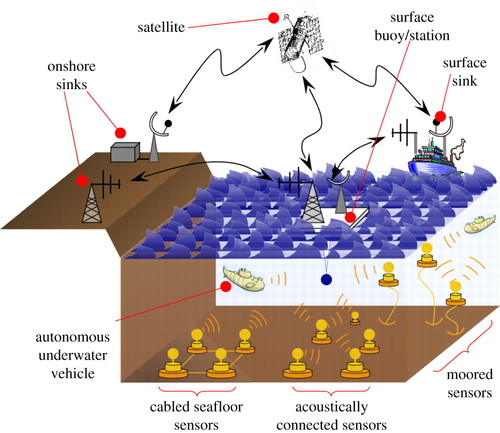
\includegraphics[width=0.8\textwidth]{underwater_network_topologies.jpg}
  \caption{Generic Underwater Network Topologies}
  \label{fig:underwater_network_topologies}
\end{figure}
\section{Basic Wireless Network Topologies}
There are 5 types of basic wireless network topologies. These are:

\begin{itemize}
\item{Point To Point}
\item{Star}
\item{Mesh}
\item{Hybrid}
\item{Daisy Chain}
\end{itemize}

\subsection{Point To Point}
A point to point network consists of simply two nodes that are connected to each
other.

\subsection{Star}
A star network (also known as a Point to Multipoint) network has a centralised
controller with nodes connected via point to point connections. In an optical
wireless network this would require the controller to have multiple transmitters
and receivers.

\subsection{Mesh}
A mesh network is where nodes are connected to some (a partial mesh) or all
(a full mesh) of the other nodes in the network.

\subsection{Hybrid}
A hybrid network combines two or more topologies.

\subsection{Daisy Chain}
A daisy chain network connects nodes in series with each other. If they are
connected all together this is known as a 'ring' network.

\subsection{Modelling - Wired versus Wireless}
In wired networks there is also a 'bus' network. However, because wireless
optical communications will be blocked by the receiver, this cannot be factored
in.

If the beam is narrow the network can be thought to act as a 'wired' network
(in that, all connections are point to point only).

If, however, the beam is wider then multiple nodes may be contactable, in which
case we can model this more akin to a wireless access point.


\begin{figure}[H]
  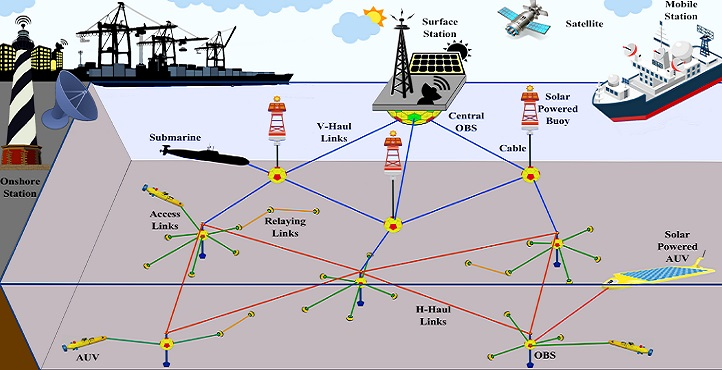
\includegraphics[width=0.8\textwidth]{underwater_network_topologies_v2.jpg}
  \caption{Generic Underwater Network Topologies}
  \label{fig:underwater_network_topologies_v2}
\end{figure}

\subsection{Underwater versus Terrestrial}
In \cite{s16030414} it is discussed that underwater topologies are highly
dynamic, due to water currents, thus the topology changes frequenctly
(compared to terrestrial networks).

Also, almost all underwater nodes would have to be powered by batteries,
so energy efficient topologies and routing protocols are necessary.

\subsubsection{Always-connected nodes}
In \cite{POMPILI2009778} it is claimed that nodes should coordinate their
depth in such as way to guarantee that the network topology is always connected.
This means there is always a path from every node to the the surface station.

\subsubsection{Tier-based modelling}
In \cite{tier_based_underwater_routing} the topology is partitioned into tiers.
Each node can only select nodes belonging to an upper tier, reducing the
complexity of routing protocols.
\section{Applications}
In order to examine underwater optical wireless network topologies
it is prudent to first examine the applications and resources that
we need to connect together.

\subsection{Dimensionality}
As described in \cite{saeed2018underwater} underwater topologies can be broken
down into 1-dimensional, 2-dimensional and 3-dimensional architectures, and also
whether they are static or mobile. However, unless they are 1-dimensional
networks, which are always star networks, the classification of the
architectures depends on the application.

\subsection{Point to Point}
Point to point is applicable in \ac{LOS} links, unless the beam has a large
beam divergence (although this will dramatically reduce the range and is
thus unpractical).

\subsection{Point to Multi-point}
Point to multi-point can only be realised by utilising \ac{NLOS} links, as
we can take advantage of scattering effects from the surface or particulate
matter in the water to communicate to multiple nodes.

\subsection{Above Surface to Underwater}
This includes nodes above the water such as on a satellite or \ac{UAV}.

\subsubsection{Relay Nodes}
This scenario is applicable for relay nodes if the above water node
can be considered 'static'. A relay node could communicate above water
using RF and underwater using an optical link.

\subsection{Surface to Underwater}
This includes nodes on the surface of the water such as on a ship
or a buoy, to nodues under the water such as \ac{ROV}s.

\subsection{Underwater to Underwater}
This is the main part of underwater wireless optical communications, and
includes divers, \ac{ROV}s, remote sensors and more.

\subsubsection{Intra-Diver versus Inter-Diver}
Currently, \ac{RF} links are utilised between a diver's gas supply and
their computer, to monitor the pressure. Optical links would not be
a good replacement as there is no line of sight between the transmitter
and receiver, and the distances are low. However, inter-diver presents
a much more interesting approach, where optical links may be better suited
if the divers are located further away from each other. This has been
demonstrated as part of the Anglerfish \ac{UOWC} system, for example.

\subsection{Static and Mobile Nodes}
As well as whether they are on the surface or under water, nodes can be
considered static (such as fixed sensors) or mobile (such as \ac{ROV}s).

\subsection{Example Applications}
\begin{itemize}
\item{Ocean Sampling Networks}
\item{Environmental Monitoring}
\item{Undersea Exploration}
\item{Disaster Prevention}
\item{Command / Control}
\item{Assisted Navigation}
\item{Distributed tactical surveillance}
\item{Mine reconnaissance}
\item{Location and Positioning}
\end{itemize}

In \cite{iout_comprehensive} these are classified into 5 categories:
\begin{enumerate}
\item{Environmental Monitoring}
\item{Underwater Exploration}
\item{Disaster Prevention}
\item{Military}
\item{Others}
\end{enumerate}
\section{Centralized versus De-Centralized}
In traditional WiFi there are two basic types of networks, a
centralized system where all stations connect
to a single access point, and a de-centralized
network where stations communicate peer-to-peer.

\subsection{Centralized}
A centralized system has a single point of failure, but allows
for simple routing as all communications go via the central
node.

\subsection{De-Centralized}
In a partial mesh we can add redundancy as at least two
nodes have two or more paths between them. This allows for packets
to be re-routed along a different path if a link fails. However, this
will require more hops for every packet, increasing latency.

\section{Comparison of Available Wireless Communication Technologies}

There are three ways to communicate wirelessly underwater. These are
acoustic, optical and \ac{RF}.

\begin{figure}[H]
  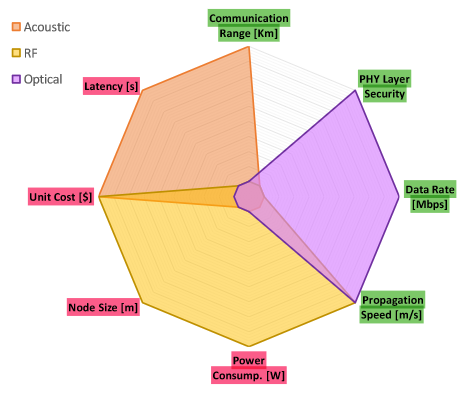
\includegraphics[width=0.8\textwidth]{acoustic_rf_optical_comparison.png}
  \caption{Comparison of Acoustic vs RF vs Optical Technologies}
  \label{fig:acoustic_rf_optical_comparison}
\end{figure}

\subsection{Above Surface to Underwater}

\subsection{Surface to Underwater}

\subsection{Hybrid Approaches}

\subsubsection{Control Plane versus Data Plane}
It is possible to utilise a hybrid approach to wireless underwater
communications. For example, we can use the much more reliable
acoustic link, which has a much lower data rate, for the control
plane. This gives reliability but a low throughput. The data plane
would then be over the optical link, giving high throughput with
much higher range than \ac{RF}.
\section{Underwater Sensor Networks}
There has been a lot of work on underwater sensor networks regarding topologies.
\section{Topology Proposals}
In order to propose topologies, we need to logically split the networks into
classes, based not just on the number of nodes but also their applications.

\begin{itemize}
\item{Point To Point}
\item{Star}
\item{Mesh}
\item{Hybrid}
\item{Daisy Chain}
\end{itemize}

\subsubsection{Point to Point}
A Point to Point topology is only suitable for a single underwater node and a
node operating on the surface, or above.

\subsubsection{Star Topology}
A star topology is suitable for the following applications:
\begin{itemize}
\item{Short Distance - Optical links can only operate over short distances thus
we can only consider these for star topologies}
\item{Two Dimensional Architecture \cite{POMPILI2009778} - Where nodes are
anchored to the bottom of the seabed and connected to the surface via a single
vertical transceiver}
\end{itemize}

\subsubsection{Daisy Chain / Mesh Topology}
Daisy chain / mesh topology is suitable for the following applications
\begin{itemize}
\item{Long Distance - A mesh would increase redudancy compared to a simplistic
chain, but increase the routing complexity and thus time delay. Daisy chain is
a simpler version that has increased time delay due to the number of hops
but less routing complexity, with no redudancy.}
\item{Three Dimensional Architecture \cite{POMPILI2009778} - where nodes float
in mid water at different heights.}
\end{itemize}

\subsubsection{Hybrid Topology}
A hybrid topology is suitable for the following applications
\begin{itemize}
\item{Three Dimensional Architctecture - A layered approach such as an inverted tree would be
suitable for a mutli-level network as described in
\cite{tier_based_underwater_routing}.}

\end{itemize}





\section{Conclusions}
This document has summarized underwater optical wireless network
topologies, their advantages, disadvantages, and discussed potential
data rates and ranges.

\section{List of Acronyms}
\begin{acronym}
\acro{AGC}{Automatic Gain Control}
\acro{APD}{Avalanche Photodiode}
\acro{BER}{Bit Error Rate}
\acro{FEC}{Forward Error Correction}
\acro{FOV}{Field Of View}
\acro{IM/DD}{Intensity Modulation / Direct Detection}
\acro{ISI}{Inter-Symbol Interference}
\acro{I2C}{Inter-Integrated Circuit}
\acro{KAUST}{King Abdullah University of Science and Technology}
\acro{LDPC}{Low Density Parity Code}
\acro{LED}{Light Emitting Diode}
\acro{LOS}{Line Of Sight}
\acro{MAC}{Medium Access Controller}
\acro{NLOS}{Non Line Of Sight}
\acro{OFDM}{Orthogonal Frequency Division Multiplexing}
\acro{OOK}{On-Off Keying}
\acro{PCIe}{Peripheral Component Interconnect Express}
\acro{PIN}{P-I-N}
\acro{PMT}{Photo Multiplier Tube}
\acro{PPM}{Pulse Position Modulation}
\acro{PWM}{Pulse Width Modulation
\acro{P2P}{Peer to Peer}
\acro{RF}{Radio Frequency}
\acro{ROV}{Remotely Operated Vehicle}
\acro{RS}{Reed-Solomon}
\acro{RSSI}{Received Signal Strength Indicator}
\acro{SFP}{Small form-factor pluggable}
\acro{SNR}{Signal to Noise Ratio}
\acro{SPAD}{Single Photo Avalanche Diode}
\acro{SPI}{Serial Peripheral Interface}
\acro{UART}{Universal asynchronous receiver/transmitter}
\acro{UOWC}{Underwater Optical Wireless Communication}
\acro{USB}{Universal Serial Bus}
\end{acronym}


\bibliographystyle{plain}
\bibliography{research}

\end{document}\grid
